\documentclass[10pt,a4paper]{article}

\usepackage[margin=2cm]{geometry}
\usepackage{booktabs}
\usepackage{longtable}
\usepackage{array}
\usepackage{graphicx}
\usepackage{xcolor}
\usepackage{enumitem}
\usepackage{tikz}
\usetikzlibrary{positioning,arrows.meta}
\usepackage[hidelinks]{hyperref}

\setlength{\parindent}{0pt}
\setlength{\emergencystretch}{2em}
\setlength{\parskip}{4pt}
\setlist{nosep,leftmargin=1.4em}
\renewcommand{\arraystretch}{1.2}

\newcolumntype{L}[1]{>{\raggedright\arraybackslash}p{#1}}
\newcommand{\ep}[1]{\texttt{\small #1}}
\DeclareUrlCommand\route{\def\UrlFont{\ttfamily\small}\def\UrlBreaks{\do\/\do-\do:\do|\do.}}

\title{\textbf{Phase 2 Documentation -- Fabulari Chat System}\\[2pt]\large 3813ICT Full Stack Development}
\author{Hadi Alkhub \quad s5331680 \quad Workshop: Wednesday 3pm\\
\small GitHub: \url{https://github.com/HadiAlk4/Chat-App-System}}
\date{October 2026}

\begin{document}
\maketitle

\section{Overview}
Fabulari is a MEAN-stack chat application: MongoDB (native Node driver), Express 5, Angular 22 (standalone components, PaperCSS) and Node.js, with Socket.io for real-time chat and live request queues. Users chat in rooms that belong to groups. Three roles, Super Admin, Group Admin (GA) and User, control what each person can see and do. Phase 1 kept most data in a JSON file or in mock arrays. In Phase 2 every screen reads and writes MongoDB through the API.

\textbf{Running it:} start MongoDB on \ep{localhost:27017}; \ep{cd backend \&\& npm start} (port 3000); \ep{cd frontend \&\& npm start} (port 4200).

\section{Specifications and Requirements}
Requirements come from the brief, the client meeting (Week 2) and the published clarifications. Status reflects the code on \ep{main}.

\begin{longtable}{L{2.6cm} L{11.2cm} L{1.9cm}}
\toprule
\textbf{Area} & \textbf{Requirement} & \textbf{Status}\\
\midrule
\endhead
Stack & MEAN stack. MongoDB replaces \ep{fakeData.json}. Socket.io handles real-time events. & Done\\
Auth & Basic email and password login. Passwords are hashed with bcrypt. OAuth is not used. & Done\\
Password rule & At least 8 characters, alphanumeric only, at least one uppercase letter. Checked on signup and password change. & Done\\
Bootstrap & The first account registered becomes the only Super Admin. Signup shows a note when the database has no users. & Done\\
Super Admin & Handles requests only. Cannot chat, read chat history, join or propose groups. Creates a group only by approving a user proposal, and the proposer becomes the first GA. Cannot delete or ban themselves. & Done\\
Global ban & Approving an account deletion removes the user and all their messages, and adds their email to a permanent ban list. Banned emails cannot log in or register again. & Done\\
Audit log & Every Super Admin decision is stored with a timestamp. A dedicated page filters by action type and date range. & Done\\
Groups & Unique group names. Any user can view all groups and request to join. No limit on how many groups a user joins or administers. & Done\\
Age limit & Min age applies to every room in the group. Users under it cannot request to join. Raising it removes members who are too young, but cannot remove the last GA. & Done\\
GA settings & Edit name, description ($\le$250 chars), min age and theme without Super Admin approval. A confirm dialog lists the changes first. & Done\\
Rooms & GA creates, renames and deletes rooms. Users propose rooms and the GA approves or rejects them. Zero to unlimited rooms per group. & Done\\
Members & GA can promote members to GA. A group always keeps at least one GA. GA sees the allowed and banned member lists. & Done\\
Group bans & Bans are permanent and there is no un-ban. Users can ask a GA to ban someone. A ban on a GA goes to the Super Admin instead. & Done\\
Step down & A GA cannot step down if they are the only GA or have pending Super Admin requests. & Done\\
Group deletion & A GA requests deletion and the Super Admin approves it. The group and its data are removed, and the GA is demoted if they administer no other group. & Done\\
Requests & Rejections need a reason. Pending requests cannot be cancelled. Users see pending and rejected requests in Request History. & Done\\
Messaging & Single-channel, single-thread. Text plus PNG, JPEG and GIF images up to 2\,MB. No external links. Shows sender name and timestamp. Users can delete their own messages. & Done\\
History & Only the last 5 messages are loaded when entering a room. Live messages are not capped while the user stays. A new room starts blank. & Done\\
Real-time & Join and leave toasts (closable with X), live participant sidebar, GA badge in the sidebar, and a toast when a join request is accepted or denied. & Done\\
Cascade delete & When an account deletion is approved, that user's messages disappear from every open chat straight away. & Done\\
Theme & The group's theme (light/dark) applies to its chat rooms. A user can override it with a personal theme that applies across all groups. & Done\\
Profile & Username (changeable), email (fixed, unique ID), password change with current password, DOB/age, role, profile picture ($\le$2\,MB), memberships. Profiles are private. & Done\\
Responsive & Desktop first and usable at tablet width (PaperCSS grid). & Done\\
HTTPS & Messages served over HTTPS. & Not done\\
\bottomrule
\end{longtable}

\textbf{Known limitations.} The server runs on HTTP. The API trusts the username sent by the client and has no session token, so role checks happen in the Angular guard and in selected routes. The upload filter also accepts WebP, which the spec does not list.

\section{Server-side API}
Base URL \ep{http://localhost:3000}. Bodies are JSON (uploads use \ep{multipart/form-data}). Most responses have the form \ep{\{ ok, message, ...data \}}. Validation failures return \ep{ok:false} with a 400, 403 or 404 status. Server errors return 500. \ep{GET} list endpoints return an array.

\subsection{REST endpoints}
\small
\begin{longtable}{L{1.5cm} L{4.9cm} L{3.2cm} L{5.6cm}}
\toprule
\textbf{Method} & \textbf{Endpoint} & \textbf{Input} & \textbf{Behaviour}\\
\midrule
\endhead
\multicolumn{4}{l}{\textit{Authentication and users}}\\
POST & \route{/api/auth} & email, password & bcrypt compare. Blocks banned emails. Returns the user without the password.\\
GET & \route{/api/signup/first-user} & -- & \ep{\{ firstUser \}}. True when no users exist yet.\\
POST & \route{/api/signup} & username, email, password, dob, age & Checks the password rule, the ban list and duplicate emails. The first user becomes \ep{super-admin}.\\
PATCH & \route{/api/users/username} & email, newUsername & Must be unique. Renames the user in groups, messages and requests.\\
PATCH & \route{/api/users/password} & email, currentPassword, newPassword & Checks the current password, then applies the rule and stores the new hash.\\
PATCH & \route{/api/users/theme} & email, isDarkMode, usePersonalTheme & Saves the personal chat theme override.\\
\midrule
\multicolumn{4}{l}{\textit{Groups, rooms and members}}\\
GET & \route{/api/groups} & -- & All groups.\\
GET & \route{/api/groups/user/:username} & -- & Groups where the user is a member or admin.\\
GET & \route{/api/groups/:groupName} & -- & One group, 404 if missing.\\
PATCH & \route{/api/groups/:groupName} & groupName, groupDescription, minAge, themeColor, username & GA only (403 otherwise). Unique name, description $\le$250 chars. Removes members under the new min age. A rename updates every collection.\\
POST & \route{/api/groups/:groupName/leave} & username & Leave the group. The only GA cannot leave.\\
POST & \route{/api/groups/:groupName/rooms/direct} & roomName & GA adds a room. Names are unique within the group, ignoring case.\\
PATCH & \route{/api/groups/:groupName/rooms/rename} & oldName, newName & Rename a room.\\
DELETE & \route{/api/groups/:groupName/rooms/:roomName} & -- & Delete a room.\\
POST & \route{/api/rooms} & groupName, roomName & Older direct add from Phase 1.\\
PATCH & \route{/api/groups/:g/members/:u/promote} & -- & Add the member to \ep{admins}.\\
POST & \route{/api/groups/:g/members/:u/remove} & -- & Remove the member. The only GA cannot be removed.\\
POST & \route{/api/groups/:g/members/:u/ban} & -- & Permanent group ban (\ep{bannedMembers}). The only GA cannot be banned.\\
POST & \route{/api/groups/:g/admins/:u/step-down} & -- & Blocked if they are the only GA or have pending Super Admin requests. Demotes their role if they administer no other group.\\
\midrule
\multicolumn{4}{l}{\textit{Request queues (each has create, list, approve, reject; reject needs \ep{reason})}}\\
POST, GET & \route{/api/group-requests} & groupName, description, minAge, themeColor, creator & Group proposal to the Super Admin. The name must be free. The Super Admin cannot propose.\\
PATCH & \route{/api/group-requests/:id/approve|reject} & performedBy, reason & Approve creates the group with a \ep{Main Room} and the proposer as GA. Both are audited.\\
POST, GET & \route{/api/join-requests} & groupName, username & Checks age, ban and duplicate requests. The Super Admin cannot join.\\
PATCH & \route{/api/join-requests/:id/approve|reject} & reason & Approve adds the user to \ep{members}.\\
POST, GET & \route{/api/room-requests} & groupName, roomName, username & Members only. The room name must be free.\\
PATCH & \route{/api/room-requests/:id/approve|reject} & reason & Approve adds the room.\\
POST, GET & \route{/api/group-ban-requests} & groupName, targetUsername, requestedBy & Routed to the GA, or to the Super Admin if the target is a GA. Filter with \ep{destination}.\\
PATCH & \route{/api/group-ban-requests/:id/approve|reject} & reason & Approve applies the permanent group ban.\\
POST, GET & \route{/api/group-deletion-requests} & groupName, requestedBy, reason & GA only. One pending request per group.\\
PATCH & \route{/api/group-deletion-requests/:id/approve|reject} & performedBy, reason & Approve deletes the group, its messages and its requests, and demotes the GA. Audited.\\
POST, GET & \route{/api/account-deletion-requests} & username & The user asks to delete their account. Not allowed for the Super Admin.\\
PATCH & \route{/api/account-deletion-requests/:id/approve|reject} & performedBy, reason & Approve deletes the user and their messages and bans the email. Audited as a global ban.\\
GET & \route{/api/banned-emails} & -- & Permanently banned emails, newest first.\\
\midrule
\multicolumn{4}{l}{\textit{Chat, uploads and audit}}\\
GET & \route{/api/messages/:groupName/:roomName} & query: username & Last 5 messages, oldest first. Returns 403 for the Super Admin.\\
DELETE & \route{/api/messages/:id} & -- & Delete a message.\\
POST & \route{/api/upload/avatar} & form: image, username & Image $\le$2\,MB. Sets \ep{profilePictureUrl}.\\
POST & \route{/api/upload/chat} & form: image & Image $\le$2\,MB. Returns \ep{fileUrl} (served from \route{/uploads}).\\
GET & \route{/api/audit-logs} & query: action, startDate, endDate & Filtered audit log, newest first.\\
\bottomrule
\end{longtable}
\normalsize

\subsection{Socket.io events}
Room channels are named \ep{groupName:roomName}. The server ignores chat events from unknown users and from the Super Admin, and drops messages that contain \ep{http(s)://} or \ep{www.}.

\small
\begin{longtable}{L{2.2cm} L{4.0cm} L{9.5cm}}
\toprule
\textbf{Direction} & \textbf{Event} & \textbf{Payload and effect}\\
\midrule
\endhead
client$\to$server & \ep{join-room}, \ep{leave-room} & \ep{\{groupName, roomName, username\}}. Joins or leaves the channel and updates who is present.\\
client$\to$server & \ep{send-message} & \ep{\{groupName, roomName, senderUserName, content, imageUrl\}}. Saves to \ep{messages}, then broadcasts it.\\
client$\to$server & \ep{delete-message} & \ep{\{groupName, roomName, messageId\}}. Deletes from MongoDB, then broadcasts.\\
server$\to$room & \ep{new-message}, \ep{message-deleted} & The saved message, or \ep{\{messageId\}}.\\
server$\to$room & \ep{user-joined}, \ep{user-left}, \ep{room-users} & Trigger toasts and the live participant list.\\
server$\to$all & \ep{<queue>-created}, \ep{<queue>-resolved} & For group, join, room, group-ban, group-deletion and account-deletion requests. Queues and Request History refresh live. \ep{join-request-resolved} triggers the accept/deny toast. \ep{account-deletion-request-resolved} removes the deleted user's messages from open chats.\\
\bottomrule
\end{longtable}
\normalsize

\section{Angular Architecture}
Standalone components with routing in \ep{app.routes.ts}. The logged-in user is kept in \ep{sessionStorage}, so each browser tab has its own login. \ep{authGuard} protects every route except login and signup. It checks \ep{expectedRole} for Super Admin pages and sends a Super Admin away from \ep{chat}, \ep{my-memberships} and \ep{group-settings}.

\subsection{Components}
\small
\begin{longtable}{L{3.5cm} L{3.4cm} L{8.8cm}}
\toprule
\textbf{Component} & \textbf{Route} & \textbf{Responsibility}\\
\midrule
\endhead
\ep{Login} & \route{/login} & Posts credentials to \route{/api/auth}, stores the user, and routes by role (Super Admin dashboard or dashboard). Shows API errors, including the banned message.\\
\ep{Signup} & \route{/signup} & Registration with age from DOB and an optional profile doodle. Shows a note when the next account will be the Super Admin.\\
\ep{Dashboard} & \route{/dashboard} & Lists and searches groups, proposes a group (modal), and requests to join. Groups the user is already in are hidden. Both actions are hidden for the Super Admin.\\
\ep{MyMemberships} & \route{/my-memberships} & The user's groups, filtered by name and role. Opens chat, settings, or leave.\\
\ep{GroupSettings} & \route{/group-settings} & GA-only tabs. \textit{General}: edit and save with a confirm dialog. \textit{Rooms}: add, rename, delete. \textit{Members}: promote, ban, banned list. \textit{Requests}: join, room and ban queues. Also step down and request deletion. Updates live over sockets.\\
\ep{RequestHistory} & \route{/request-history} & The user's pending and rejected requests with reasons. Tabs to propose a room and to request a ban.\\
\ep{Chat} & \route{/chat} & Room list, last-5 history plus live messages, image attachments, delete own message, toasts, participant sidebar with GA badge, and the group or personal theme.\\
\ep{UserProfileSettings} & \route{/user-profile-settings} & Change username, password and theme. Upload a profile picture. Request account deletion.\\
\ep{SuperAdminDashboard} & \route{/super-admin-dashboard} & Live queues for group proposals, GA ban requests, group deletions and account deletions, plus the banned-email list. Every rejection needs a reason.\\
\ep{SuperAdminAuditLog} & \route{/super-admin-audit-log} & Audit table filtered by action type and date range.\\
\bottomrule
\end{longtable}
\normalsize

\subsection{Services}
\begin{itemize}
\item \ep{AuthService}: get, set and clear the session user; logout.
\item \ep{GroupService}: all group, room and member endpoints, plus every request queue (group, join, room, ban, deletion).
\item \ep{ChatService}: room history over HTTP. Emits and listens to chat socket events (\ep{join-room}, \ep{send-message}, \ep{new-message}, \ep{room-users}, and so on).
\item \ep{SocketService}: typed observables for every \ep{*-created} and \ep{*-resolved} request event.
\item \ep{AccountService}: account deletion requests, banned emails, and username, password and theme updates.
\item \ep{UploadService}: avatar and chat image uploads (\ep{FormData}).
\item \ep{AuditService}: audit log query with filters.
\end{itemize}

\subsection{Models (TypeScript interfaces)}
{\raggedright \ep{Group}, \ep{GroupRequest}, \ep{JoinRequest}, \ep{RoomRequest}, \ep{GroupBanRequest}, \ep{GroupDeletionRequest}, \ep{AccountDeletionRequest}, \ep{BannedEmail}, \ep{AuditLog}, \ep{ChatMessage}. They mirror the MongoDB documents in Section~\ref{sec:data}. Request models share a \ep{status} of \ep{pending}, \ep{approved} or \ep{rejected}, plus \ep{createdAt}, \ep{reviewedAt} and \ep{rejectionReason}.\par}

\section{Design Documents}
\subsection{System architecture}
\begin{center}
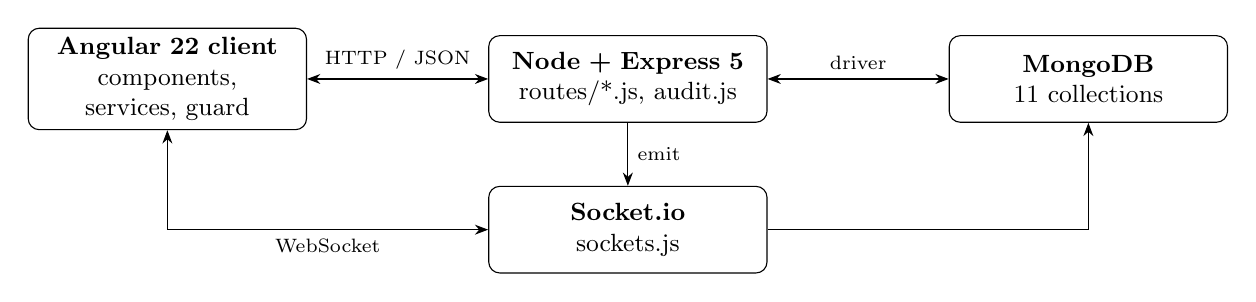
\begin{tikzpicture}[node distance=1.2cm and 2.3cm, box/.style={draw,rounded corners,align=center,minimum height=1.1cm,text width=3.3cm,font=\small}, >={Stealth}]
\node[box] (ng) {\textbf{Angular 22 client}\\components, services, guard};
\node[box,right=of ng] (ex) {\textbf{Node + Express 5}\\routes/*.js, audit.js};
\node[box,right=of ex] (db) {\textbf{MongoDB}\\11 collections};
\node[box,below=0.8cm of ex] (io) {\textbf{Socket.io}\\sockets.js};
\draw[<->] (ng) -- node[above,font=\scriptsize]{HTTP / JSON} (ex);
\draw[<->] (ex) -- node[above,font=\scriptsize]{driver} (db);
\draw[<->] (ng) |- node[pos=0.75,below,font=\scriptsize]{WebSocket} (io);
\draw[->] (ex) -- node[right,font=\scriptsize]{emit} (io);
\draw[->] (io) -| (db);
\end{tikzpicture}
\end{center}
\ep{app.js} builds the Express app (\ep{createApp(io)}). \ep{index.js} attaches the HTTP server and Socket.io. Because of this split, tests can import the app without starting a server, using a stub \ep{io}. Business rules are pulled out into small, pure helpers in \ep{backend/lib/} (password policy, age check, link check, last-5 window).

\subsection{Data structures (MongoDB collections)}\label{sec:data}
\small
\begin{longtable}{L{3.8cm} L{12.0cm}}
\toprule
\textbf{Collection} & \textbf{Fields}\\
\midrule
\endhead
\ep{users} & username, email (unique ID), password (bcrypt), dob, age, role (\ep{super-admin}|\ep{group-admin}|\ep{user}), valid, isDarkMode, usePersonalTheme, profilePictureUrl\\
\ep{groups} & groupName (unique), groupDescription, minAge, themeColor (\ep{light}|\ep{dark}), admins[], members[], rooms[], bannedMembers[]\\
\ep{messages} & groupName, roomName, senderUserName, content, imageUrl, timestamp\\
\ep{groupRequests} & groupName, groupDescription, minAge, themeColor, creatorUserName, creatorEmail + request fields\\
\ep{joinRequests} & groupName, username + request fields\\
\ep{roomRequests} & groupName, roomName, username + request fields\\
\ep{groupBanRequests} & groupName, targetUsername, targetEmail, targetRole, requestedBy, requestedByRole, destination (\ep{group-admin}|\ep{super-admin}) + request fields\\
\ep{groupDeletionRequests} & groupName, requestedBy, requestedByRole, reason + request fields\\
\ep{accountDeletionRequests} & username, email, role + request fields\\
\ep{bannedEmails} & email, username, bannedAt, reason\\
\ep{auditLogs} & timeStamp, actionPerformed, target, performedBy (insert only)\\
\bottomrule
\end{longtable}
\normalsize
\textit{Request fields} are status, createdAt, reviewedAt and rejectionReason. Groups store room names and usernames as arrays instead of references, so a single read loads a whole group. When a user or group is renamed, the server updates the name in every collection.

\subsection{Storyboards}
The Phase 1 storyboards (desktop and tablet) still describe the layout, so they were kept. They are in Appendix~\ref{app:story} and in \ep{assignment\_material/Fabulari Design/}. Changes made in Phase 2:
\begin{itemize}
\item The Group Settings \textit{General} tab is a real form and asks for confirmation before saving.
\item Request History has a \textit{Request Ban} tab.
\item The Super Admin dashboard has live GA ban and group deletion queues.
\item Chat has image attachments and a delete button on your own messages.
\item Every Super Admin rejection asks for a reason.
\end{itemize}

\section{Testing}
\subsection{Tools and methodology}
\begin{itemize}
\item \textbf{Backend unit tests}, Mocha with Node \ep{assert} (\ep{npm run unitTest}). Test the pure helpers in \ep{backend/lib}.
\item \textbf{Backend integration tests}, Mocha, Chai and chai-http (\ep{npm test}). Each test calls \ep{createApp()} against a separate \ep{chat-app-test} database. The database is wiped before and after every test, so no test depends on another. Each endpoint has at least one success case and one failure case.
\item \textbf{Angular unit tests}, Vitest with TestBed via \ep{ng test}. Services are replaced with test doubles, so components are tested without a backend.
\item \textbf{End-to-end tests}, Cypress (\ep{npm run cypress:run}), against the real frontend and a backend started with \ep{MONGO\_DB\_NAME=chat-app-test}. A \ep{resetDb} task drops the test database before each spec.
\end{itemize}
Before any tests were written, the logic was moved into testable helpers and the app setup was split from \ep{listen()}. The end-to-end tests found four screens that did not refresh after data loaded (login errors, dashboard, memberships, chat), and these were fixed.

\textbf{Results (run 1 Oct 2026):} backend unit 14/14 passing, backend integration 100/100 passing, Angular 27/27 passing. Cypress has 9 specs.

\subsection{Automated tests}
\small
\begin{longtable}{L{1.8cm} L{4.2cm} L{0.5cm} L{8.8cm}}
\toprule
\textbf{Suite} & \textbf{Target} & \textbf{\#} & \textbf{Cases}\\
\midrule
\endhead
Unit & \ep{isValidPassword} & 4 & accepts valid; rejects too short, no uppercase, symbol\\
Unit & \ep{isUnderMinAge} & 3 & under min; equal to min; missing age not treated as under\\
Unit & \ep{containsExternalLink} & 3 & detects http, www; allows plain text\\
Unit & \ep{latestMessagesOldestFirst} & 4 & keeps latest 5; exactly 5; fewer than 5; oldest-first order\\
\midrule
Integration & \route{/api/auth}, \route{/api/signup} & 6 & valid login; wrong password; banned login; first user is Super Admin; weak password; banned email signup\\
Integration & \route{/api/users/*} & 6 & rename; missing name; change password; wrong current password; save theme; missing theme flags\\
Integration & \route{/api/groups*} & 11 & list all / empty; user groups / none; get one / 404; leave / missing username; save settings and remove under-age members; missing description; non-GA 403\\
Integration & rooms & 8 & add / missing name; rename / missing new name; delete / 404; \ep{POST /api/rooms} add / unknown group\\
Integration & members & 8 & promote / 404; remove / only GA; ban / 404; step down / only GA\\
Integration & group requests & 8 & create / missing fields; list / empty filter; approve creates group with GA / not pending; reject with reason / no reason\\
Integration & join requests & 8 & create / under age; list / empty filter; approve adds member / not pending; reject with reason / no reason\\
Integration & room requests & 8 & create / missing fields; list / empty filter; approve adds room / not pending; reject with reason / no reason\\
Integration & group ban requests & 8 & create / missing fields; list by destination / empty; approve bans / 404; reject with reason / no reason\\
Integration & group deletion & 8 & create / missing reason; list / empty; approve deletes and demotes / 404; reject with reason / no reason\\
Integration & account deletion, banned emails & 10 & create / Super Admin blocked; list / empty; approve deletes and bans / 404; reject with reason / no reason; banned list / empty\\
Integration & \route{/api/messages} & 5 & last 5 oldest first; missing username 400; Super Admin 403; delete / 404\\
Integration & \route{/api/upload/*} & 4 & avatar PNG / no file; chat PNG / no file\\
Integration & \route{/api/audit-logs} & 2 & returns logs; filters by action\\
\midrule
Angular & \ep{App} & 2 & creates root; renders router outlet\\
Angular & \ep{authGuard} & 3 & logged out to login; user blocked from Super Admin page; Super Admin blocked from chat\\
Angular & \ep{Login} & 3 & empty fields no HTTP; user to dashboard; Super Admin to Super Admin dashboard\\
Angular & \ep{Signup} & 4 & age for past, empty and future DOB; empty form not posted\\
Angular & \ep{Dashboard} & 2 & proposal sent via service; joined groups hidden\\
Angular & \ep{Chat} & 3 & link not sent; plain text sent; history shows sender name\\
Angular & \ep{GroupSettings} & 4 & form filled from group; confirm before raising min age; rejection needs reason; non-GA redirected\\
Angular & \ep{RequestHistory}, \ep{MyMemberships} & 2 & renders a join request; renders a membership\\
Angular & \ep{SuperAdminDashboard} & 1 & renders pending proposals\\
Angular & \ep{SuperAdminAuditLog} & 2 & renders logs; applies action and date filters\\
Angular & \ep{UserProfileSettings} & 1 & shows error on wrong current password\\
\midrule
E2E & \ep{login.cy.ts} & 3 & logs in and fills dashboard; sends credentials to API; error on empty submit\\
E2E & \ep{access.cy.ts} & 3 & logged-out redirect; logged-in reaches dashboard; bad credentials stay on login\\
E2E & \ep{admin-group.cy.ts} & 1 & Super Admin approval makes the group visible to its creator\\
E2E & \ep{chat.cy.ts} & 2 & two users: other member's message shows their name; link message not shown\\
\bottomrule
\end{longtable}
\normalsize

\section{Git Workflow}
Every feature was built on its own branch and merged into \ep{main} through a GitHub pull request (221 commits, PRs \#1 to \#52). Each PR description lists what the branch changed. Phase 2 branches, in order:

\small
\begin{longtable}{L{5.8cm} L{10.3cm}}
\toprule
\textbf{Branch (PR)} & \textbf{Work}\\
\midrule
\endhead
\ep{feature/auth-route-guard} (\#28) & AuthService, route guard with roles, logout on every screen\\
\ep{feature/auth-and-live-groups} (\#30, \#31) & bcrypt and Super Admin bootstrap, Group models and service, dashboard loads live groups\\
\ep{feat/group-proposal-flow} (\#32, \#33) & Group proposal to Super Admin queue; first Socket.io events\\
\ep{feature/group-join-requests} (\#34, \#35) & Join request model, routes, sockets, GA queue, Request History\\
\ep{refactor/backend-mongodb-structure} (\#36) & Split backend into \ep{db.js} and \ep{routes/*} modules\\
\ep{feat/room-proposal} (\#37, \#38) & Room proposals wired to Group Settings\\
\ep{feature/my-memberships} (\#39) & Memberships from MongoDB\\
\ep{feature/group-settings} (\#40) & Rooms and Members tabs on live data\\
\ep{feat/chat} (\#41, \#42) & Messages collection, chat sockets, last-5 history, delete, live participants\\
\ep{feature/file-attachments} (\#43) & Multer uploads for avatars and chat images\\
\ep{account-deletion-bans} (\#44) & Account deletion queue, permanent email bans\\
\ep{audit-log-mongodb} (\#45) & Audit log collection and filtered page\\
\ep{user-profile-mdb} (\#46) & Username, password and theme updates\\
\ep{group-admin-remaining} (\#47) & Unique names, settings save, age eviction, group bans, ban requests, step down, group deletion\\
\ep{feat/sa-request-only-scope} (\#48) & Super Admin limited to requests (UI, guard, API, sockets)\\
\ep{feat/chat-toast-cascade-theme} (\#49) & Join toasts, live cascade delete, link blocking, personal theme\\
\ep{testing} (\#50) & Testable refactor, then Mocha, Chai, Vitest and Cypress suites\\
\ep{cleanup-bugs} (\#51, \#52) & GA check on settings, confirm dialog, first-user note, per-tab sessions\\
\bottomrule
\end{longtable}
\normalsize

\appendix
\section{Storyboards}\label{app:story}
\begin{center}
\newcommand{\storyboard}[2]{\begin{minipage}[t]{0.48\textwidth}\centering\includegraphics[width=\linewidth,height=6.3cm,keepaspectratio]{figures/#1}\\\small #2\end{minipage}}
\storyboard{login-signup.pdf}{Login / Sign up}\hfill\storyboard{dashboard.pdf}{Dashboard}\\[8pt]
\storyboard{my-memberships.pdf}{My Memberships}\hfill\storyboard{group-settings.pdf}{Group Settings}\\[8pt]
\storyboard{request-history.pdf}{Request History}\hfill\storyboard{chat.pdf}{Chat}\\[8pt]
\storyboard{account-settings.pdf}{Account Settings}\hfill\storyboard{super-admin-dashboard.pdf}{Super Admin Dashboard}\\[8pt]
\storyboard{audit-log.pdf}{Super Admin Audit Log}
\end{center}

\end{document}
